\section{Generative Adversarial Networks}
This is an hyped field, but first we need some background regarding autoencoders.

\subsection{Autoencoder}
An \textbf{autoencoder} is a network which is meant to learn a sort of identity mapping; you are given an input of input neurons and you train a network which has as output some output neurons and the output is meant to be exactly the same input. The first part that goes from the input to the bottleneck is called \textbf{encoder}, while in output you have the \textbf{decoder}.  
\begin{center}
    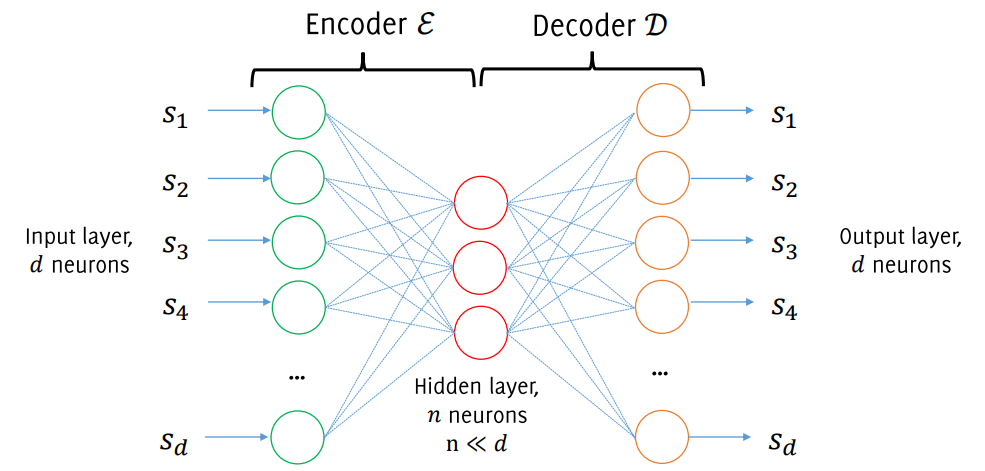
\includegraphics[width=0.75\textwidth]{images/autoencoder.PNG}\par
\end{center}
This seems some stupid task because you are already given the input and you are trying to learn a neural network to transform the input into itself. The autoencoders are used, for example, for data reconstruction. An autoencoder is a type of artificial neural network used to learn efficient data codings in an unsupervised manner. The aim of an autoencoder is to learn a representation (encoding) for a set of data, typically for dimensionality reduction, by training the network to ignore signal “noise”. Indeed, you can design your network to have a bottleneck of much fewer neurons than the input, so you learn a function that compresses our input signal to a lower dimension representation, it's a more compact representation of the input signal. \\
So Autoencoders are non-parametric models that can be trained to reconstruct all the data in a training set. The reconstruction loss is:
\begin{center}
    $\sum_{s \in S}\|s-\mathcal{D}(\mathcal{E}(s))\|_{2}$
\end{center}
The training of $\mathcal{D}(\mathcal{E}(\cdot))$ is done via standard backpropagation algorithms. This is important in the context of having a latent representation of object; with autoencoders you want to learn a \textit{latent representation} which is meant to provide a compact representation of your input which allows to recover the signal (it's like setting a 1-to-1 correspondence).

You can use these autoencoders also in CNN., for example segmentation networks are similar to the architecture of autoencoders. You can train convolutional autoencoders to find some compressed representation removing the noise. \\

Remarks:
\begin{itemize}
    \item[--] Features $z$ are typically referred to as \textbf{latent representation}
    \item[--] Autoencoders typically do not provide exact reconstruction since $n << d$, by doing so we expect the latent representation to be a meaningful and compact representation of the input
    \item[--] Additional \textit{regularization terms} might be included in the loss function
    \item[--] More powerful and non-linear representation can be learned by \textit{stacking multiple hidden layers} (deep architectures)
\end{itemize}{}

These are also useful to perform in practice to provide a \textbf{good initialization} to a network. As soon as you are given a huge amount of train images which are sort of unlabeled (imagine a semi-supervise setting), a way to learn also from not annotated images is the following:
\begin{enumerate}
    \item first you train, using not annotated images, an autoencoder which tries to reconstruct your input, in a fully unsupervised way;
    \item once you have trained the autoencoder, you get rid of the decoder and you keep the compressed representation;
    \item than if you are given some training samples, you plug in the rest of your network for classification purposes and you fine-tune the full network on the training samples. 
\end{enumerate}
In this case you are also able to exploit an unsupervised problem to provide a good initialization and prevent the risk of overfitting. The feature that you learn for reconstruction may not be too good for classification but in principle the first they should be good for the first convolutional features.\\

Autoencoders provide a \textit{good initialization} (and reduce the risk of overfitting) because their latent vector is actually a good representation of the inputs used for training. 

\subsection{Generative Models: Variational Autoencoders}
\textbf{Goal} Generative models generate, given a training set of images (data) $S$, other images (data) that are similar to those in $S$. \\

Generative models can be used for \textit{data augmentation}, simulation and planning. \\
Training generative models can also enable inference of latent representation that can be useful as general features. \\

What about using Autoencoders as Generative Models? \\
The important thing for us in this case is the latent representation that we get from an autoencoder. This latent representation is good at describing images but wouldn't be good at generating images. Given an image I can compress and decompress it, so one option could be to take the decoder network $\mathcal{D}$ and discard the encoder. Variational autoencoders leverage a prior distribution learnt by the autoencoders over $z$ to generate images with an architecture similar to this. \\
The procedure: 
\begin{enumerate}
    \item Train an autoencoder on $S$
    \item Discard the encoder
    \item Draw random vectors to replace the latent representation and feed this to the decoder input
\end{enumerate}
\begin{center}
    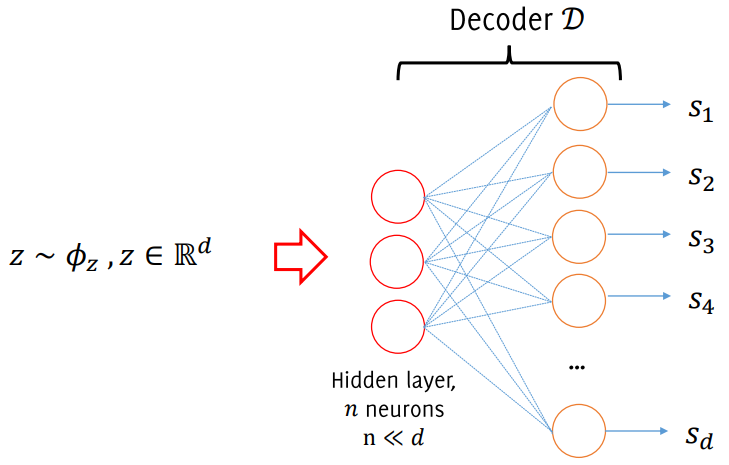
\includegraphics[width=0.6\textwidth]{images/autogenerative.PNG}\par
\end{center}
Unfortunately this does not work, you cannot randomly generate an image by just throwing some random numbers inside the latent representation. The problem is that we don't know the distribution of proper latent representation (or it's very difficult to estimate it). The goal is to find out a way to randomly generate images that actually look like a real image, an image with a meaning. This task was solved by \textbf{Generative Adversarial Networks}.

\subsection{Generative Models: GANs}
We are not looking for an explicit density model $\phi_{s}$ describing the "secret" manifold of natural images, we just want to find out a model able to generate samples that look like training samples.

Instead of sampling from $\phi_{s}$, just:
\begin{itemize}
    \item[--] Sample a seed from a known distribution $\phi_{z}$
    \item[--] Feed this seed to a learned transformation that generates realistic samples, as if they were drawn from $\phi_{s}$
\end{itemize}{}
We will be given some sort of random distribution $\phi_{z}$ which is a uniform distribution over a $d$-dimensional space. From the distribution we sample a seed $z$, which is a random number with $d$ components and $\phi_z$ is the distribution used to generate this number.\\
Now what I would like to do is to train a network $\mathcal{G}$ that takes as input $z \sim \phi_{z}, z \in \mathbb{R}^{d}$ and provides me $\mathcal{S}$ which is a "nice" image and of course belongs to $\mathbb{R}^{n}$, in particular it belongs to the secret manifold of images. In general what I want is taking a random noise, feed it to a generative network and obtain an image like this that's randomly generated:
\begin{center}
    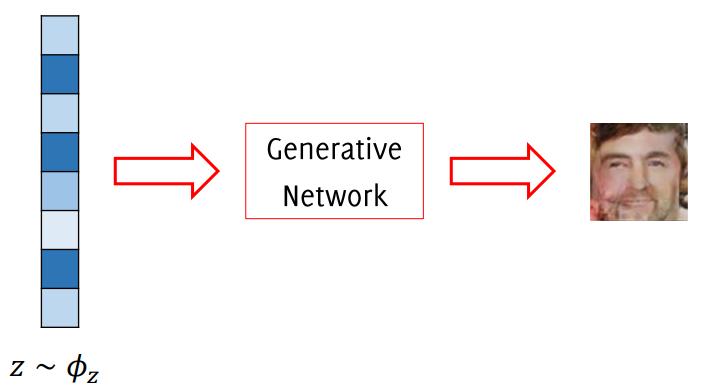
\includegraphics[width=0.6\textwidth]{images/gan_vecchio.PNG}\par
\end{center}
If you change the noise, you get a different image. 

Why is this problem challenging?\\
What misses here is an \textit{appropriate loss function}. The loss function should tell how "happy" we are with the output image, and being happy means that the image looks like a natural image. Obviously this is hard to measure because you need a number, so the trick of GANs was to replace this loss with another neural network, called \textbf{discriminator} $\mathcal{D}$.\\
The discriminator network $\mathcal{D}$ is trained to determine if the images generated by the generator network $\mathcal{G}$ are real, to classify between real and fake images. 

Thus, The GAN solution is to train a pair of neural networks with different tasks that compete in a sort of two player game.\\
The models are:
\begin{itemize}
    \item \textbf{Generator} $\mathcal{G}$ that produces realistic samples e.g. taking as input some random noise. $\mathcal{G}$ tries to fool the discriminator
    
    \item \textbf{Discriminator} $\mathcal{D}$ that takes as input an image and assess whether it is real or generated by $\mathcal{G}$
\end{itemize}{}
Train the two model and at the end, keep only $\mathcal{G}$ \\

The key idea is that instead of having a measure of how much our image looks like a natural image, you train another network simultaneously which in this context operates like a loss function. After a successful GAN training, the discriminator $\mathcal{D}$ is completely useless because it is no longer able to distinguish between real and fake images and the generator is able to cheat the discriminator, so we throw it away and we take only the generator $\mathcal{G}$.

Let's write this formally. Let's call $\mathcal{G}$ the generator and $\mathcal{D}$ the discriminator.
\begin{center}
    $\mathcal{D}=\mathcal{D}\left(\boldsymbol{s}, \theta_{d}\right)$ \\
    $\mathcal{G}=\mathcal{G}\left(\mathbf{z}, \theta_{g}\right)$
\end{center}
(\textbf{Note} that the role of n and d are reversed: from now on, n is the size of an image and d is the size of the input noise)\\
 These networks will have some parameters $\theta_{d}$ and $ \theta_{g}$, $\boldsymbol{s}\in \mathbb{R}^{n}$ is an input image (either real or generated by $\mathcal{G}$) and $\boldsymbol{z}\in \mathbb{R}^{d}$ is some random noise to be fed to the generator network. 
 Our network gives as output:
\begin{itemize}
    \item[--] The posteriori for an input to be a true image: $
\mathcal{D}\left(\cdot, \theta_{d}\right): \mathbb{R}^{n} \rightarrow[0,1]
$
    \item[--] The generated image: $
\mathcal{G}\left(\cdot, \theta_{g}\right): \mathbb{R}^{d} \rightarrow  \mathbb{R}^{n}
$
\end{itemize}{}
A good discriminator is such: 
\begin{itemize}
    \item $\mathcal{D}\left(\boldsymbol{s}, \theta_{d}\right)$ is maximum when $s \in S$
    \item $ 1 - \mathcal{D}\left(\boldsymbol{s}, \theta_{d}\right)$ is maximum when $s$ was generated from $\mathcal{G}$
    \item $ 1 - \mathcal{D}\left(\mathcal{G}\left(\boldsymbol{z}, \theta_{g}\right), \theta_{d}\right)$ is maximum when $\boldsymbol{z} \sim \phi_z $
\end{itemize}{}
 When training $\mathcal{D}$ we try to maximize the binary cross-entropy, the classification accuracy, so training $\mathcal{D}$ means solving this classification problem:
 \begin{center}
     $\max _{\theta_{d}}\left(\mathrm{E}_{s \sim \phi_{S}}\left[\log \mathcal{D}\left(\boldsymbol{s}, \theta_{d}\right)\right]+\mathrm{E}_{z \sim \phi_{Z}}\left[\log \left(1-\mathcal{D}\left(G\left(\mathbf{z}, \theta_{g}\right), \theta_{d}\right)\right)\right]\right)$
 \end{center}
$\mathrm{E}_{s \sim \phi_{S}}$ is the expectation, which is replaced in practice by an average over mini-batch, of $S$ drawn from $\phi_{S}$ (the distribution of natural images),  so this is the expectation over the distribution of natural images. When images are drawn from the manifold you want the first probability part to be large, while you want the probability to be small when images are drawn from the fake distribution (when they are generated by $\mathcal{G}$). The first term is the probability that the discriminator gives to an image that is true, so you want this to as close as possible to 1:
\begin{itemize}
    \item $\mathrm{E}_{s \sim \phi_{S}} [\log \mathcal{D}\left(\boldsymbol{s}, \theta_{d}\right)] $ has to be 1 since $s \sim \phi_S$, thus images are real
\end{itemize}{}
$\mathrm{E}_{z \sim \phi_{Z}}$ is the expectation over the fake distribution generated by the generator network. The second term is the probability that you want to be zero because that image is not a natural image. 
\begin{itemize}
    \item $\mathrm{E}_{z \sim \phi_{Z}} [\log ( 1 -  \mathcal{D}\left(\mathcal{G} (\boldsymbol{z}, \phi_g), \theta_{d}\right)] $ has to be 0 since $\mathcal{G} (\boldsymbol{z}, \phi_g)$ is a generated (fake) image
\end{itemize}{}
You train the neural network to maximize this sum which is the sum of the probabilities for real images and one minus the probability of fake images. \\

Now let's move to $\mathcal{G}$: a good generator $\mathcal{G}$ is the one which makes $\mathcal{D}$ \textbf{to fail}. \\
A good loss for $\mathcal{G}$ would be something that tells that the discriminator fails because we are trying to trick the discriminator providing fake images that seem real, it's a two player game. We'd like to find the parameter $\theta_{g}$ in order to minimize this:
\begin{center}
    $\min _{\theta_{g}} \max _{\theta_{d}}\left(\mathrm{E}_{S \sim \phi_{S}}\left[\log \mathcal{D}\left(\mathbf{s}, \theta_{d}\right)\right]+\mathrm{E}_{z \sim \phi_{Z}}\left[\log \left(1-\mathcal{D}\left(G\left(\mathbf{z}, \theta_{g}\right), \theta_{d}\right)\right)\right]\right)$
\end{center}
The generator should minimize the effectiveness of the discriminator. It's a min-max optimization, you have to perform the optimization simultaneously but typically it is difficult to solve directly, so what you do in practice is alternate: 
\begin{enumerate}
    \item First you do $k$-steps of SGA (in this case you perform the ascent gradient obviously) maximizing the discriminator function taking $\mathcal{G}$ fixed and optimize for $\mathcal{D}$
    $$ \max _{\theta_{d}}\left(\mathrm{E}_{S \sim \phi_{S}}\left[\log \mathcal{D}\left(\mathbf{s}, \theta_{d}\right)\right]+\mathrm{E}_{z \sim \phi_{Z}}\left[\log \left(1-\mathcal{D}\left(G\left(\mathbf{z}, \theta_{g}\right), \theta_{d}\right)\right)\right]\right)$$
    
    \item Then  you take $1$-step of SGD  maximizing the generator function taking $\mathcal{D}$ fixed and optimize for $\mathcal{G}$
    $$ \min _{\theta_{g}}\left(\mathrm{E}_{S \sim \phi_{S}}\left[\log \mathcal{D}\left(\mathbf{s}, \theta_{d}\right)\right]+\mathrm{E}_{z \sim \phi_{Z}}\left[\log \left(1-\mathcal{D}\left(G\left(\mathbf{z}, \theta_{g}\right), \theta_{d}\right)\right)\right]\right)$$
    
    we can remove the first term because it does not depend on $\theta_g$:
    $$ \min _{\theta_{g}}\left(\mathrm{E}_{z \sim \phi_{Z}}\left[\log \left(1-\mathcal{D}\left(G\left(\mathbf{z}, \theta_{g}\right), \theta_{d}\right)\right)\right]\right)$$
    
    Nothing changes if we use Gradient Ascent instead of Gradient Descent unless for the change from $min$ to $max$: 
    $$ \min _{\theta_{g}}\left(\mathrm{E}_{z \sim \phi_{Z}}\left[\log \left(1-\mathcal{D}\left(G\left(\mathbf{z}, \theta_{g}\right), \theta_{d}\right)\right)\right]\right) \longrightarrow \max _{\theta_{g}}\left(\mathrm{E}_{z \sim \phi_{Z}}\left[\log \left(\mathcal{D}\left(G\left(\mathbf{z}, \theta_{g}\right), \theta_{d}\right)\right)\right]\right)$$
    
    This change does not modify the global solution of the min-max problem, but provides a stronger gradient during the early learning stages.
\end{enumerate}
%first you do $k$-steps of SGA (in this case you perform the ascent gradient obviously) maximizing the discriminator function and then you take $1$-step of SGD  maximizing the generator function, so you leave $\mathcal{G}$ fixed and optimize for $\mathcal{D}$ and then you leave $\mathcal{D}$ fixed and optimize for $\mathcal{G}$. Once $\mathcal{D}$ is fixed after $k$-steps you only have to minimize, this means that you can have one step of SGD, and you alternate between the two.\\
Moreover, in order to achieve convergence, instead of  $\min \nabla_{\theta_{g}}\left[\sum_{i} \log \left(1-\mathcal{D}\left(\mathcal{G}\left(\mathbf{z}_{i}, \theta_{g}\right), \theta_{d}\right)\right)\right]$, it's better to  %minimize
$\max \nabla_{\theta_{g}}\left[\sum_{i} \log \left(\mathcal{D}\left(\mathcal{G}\left(\mathbf{z}_{i}, \theta_{g}\right), \theta_{d}\right)\right)\right]$.

Summing up, for $k$ times you draw a minibatch of noise realizations $z$, you sample a minibatch of images and then you update $\mathcal{D}$ by SDA; then you draw a minibatch only of noise realizations and you just update $\mathcal{G}$ by SDG, which in practice is SGA for what we just said about convergence. \\

\begin{minipage}{\linewidth}
\centering
\hspace*{-2cm}    
\begin{minipage}{9cm}
  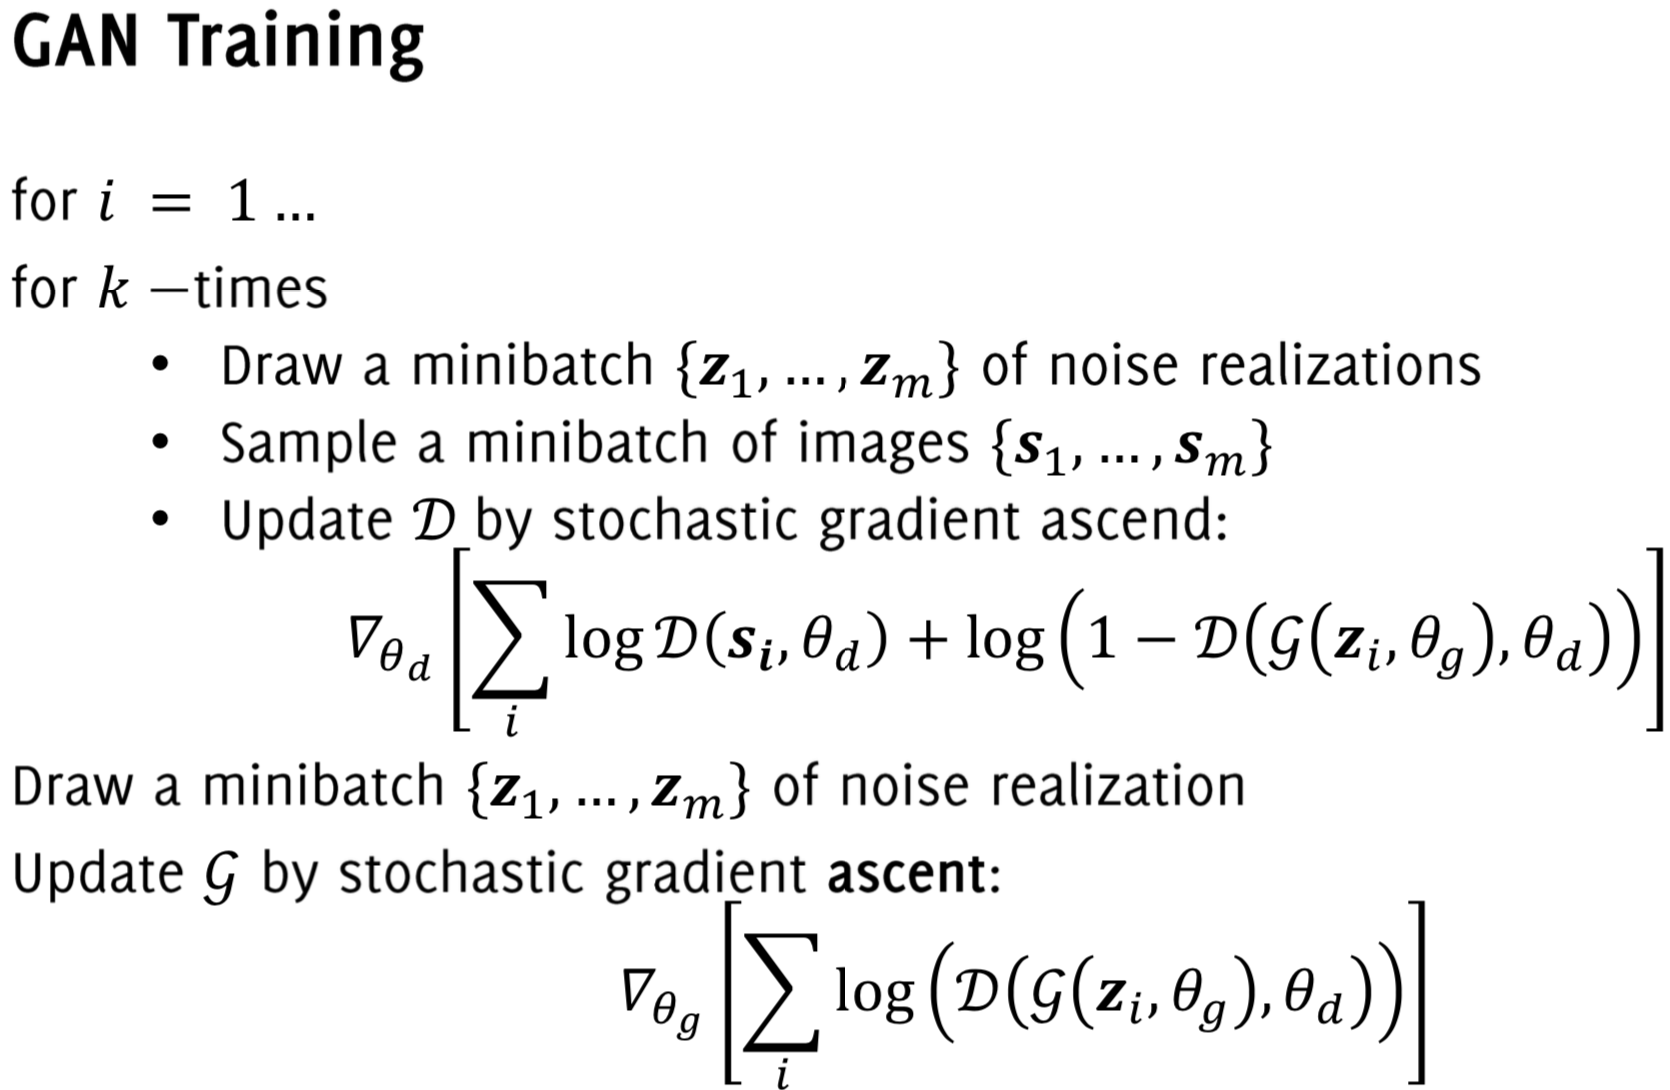
\includegraphics[width=9cm, height=7cm]{images/gan_sgd.png}
  %\captionof{figure}{A figure}
  %\label{fig:test1}
\end{minipage}%
\begin{minipage}{10cm}
  \centering
  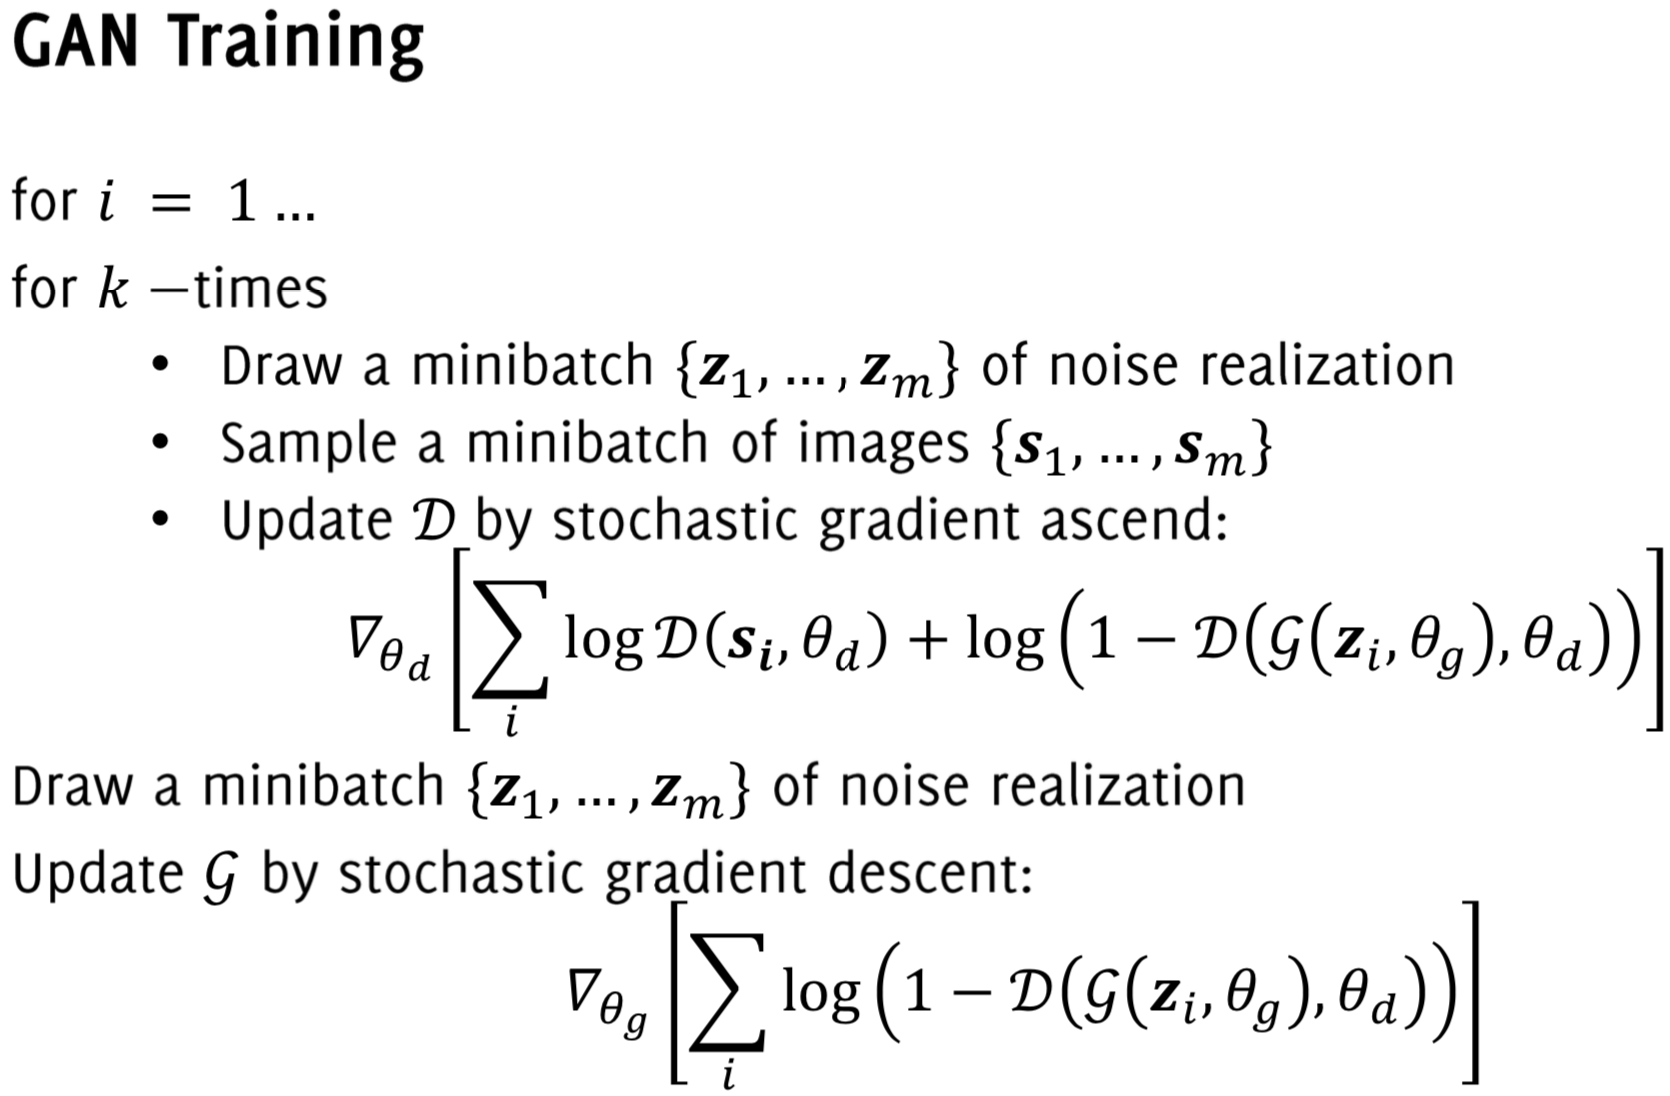
\includegraphics[width=9cm, height=7cm]{images/gan_sga.png}
  %\captionof{figure}{Another figure}
  %\label{fig:test2}
\end{minipage}
\end{minipage}\\ \\

This illustration shows how the training proceeds:
\begin{center}
    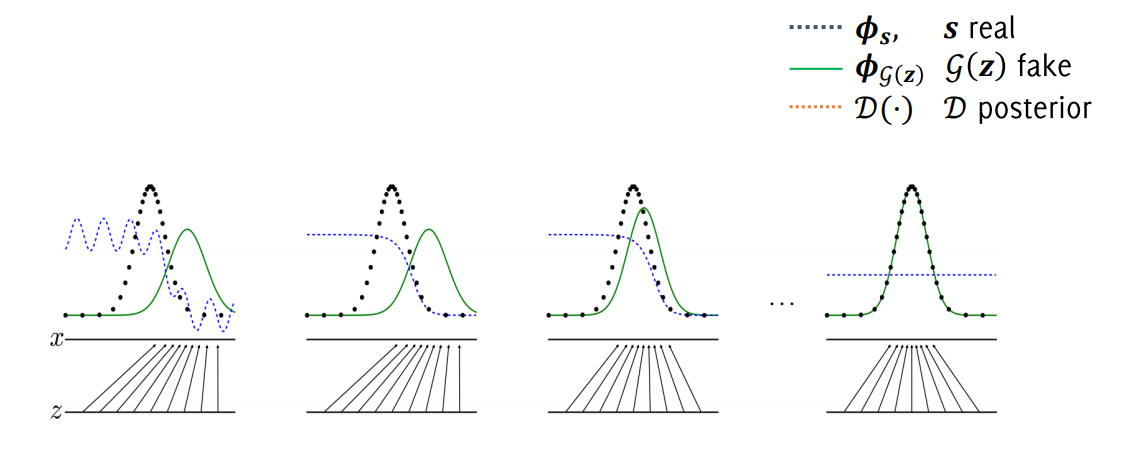
\includegraphics[width=0.8\textwidth]{images/gan_training.PNG}\par
\end{center}
Again $\phi_{s}$ is the real manifold where natural images live, it's what you want to be able to sample, and $\phi_{z}$ is the distribution of noise which are feed to the generator to get an image. At the very beginning, the images that you generate are very far from the natural images. When training better $\mathcal{D}$ you are defining better the separation between the two classes, the one generated by the network and the one of real images; but now when you are training $\mathcal{G}$, what you do is steering your generator network to provide images that are more realistic and closer to the distribution of real images. As the training proceeds, the two distribution finally overlap and the discriminator gives 0.5 probability (random probability) because it can no longer distinguish between real and fake. This is \textbf{unstable to train} but it's trained by standard tools: backpropagation and dropout. What is important is that the generator does not use directly $\mathcal{S}$ for training, it just takes as input random noise and the real images are just used in order to define some sort of loss through the game with the discriminator.\\
Generator performance is difficult to assess quantitatively. There is \textbf{no explicit} expression for the generator, it is provided in an \textbf{implicit} form $\rightarrow$ you cannot compute the likelihood of a sample w.r.t. the learned GAN